\label{sec:intro}

The models for computing the orbits for Sag are summarized in table 1.

\begin{table}[H]
\begin{center}
\begin{tabular}{c c c c c}
\hline
\textbf{MW} & Model & Mass [$M_{\odot}$] &  & \\
\hline
DM halo & NFW & $M_{vir} = 1E12$ &$R_{vir} = 261$ &  $r_s = 26.47$ \\
Disk & Miyamoto-Nagai &  $M_d = 6.5E10$ & $r_a = 3.5$ &  $r_b=0.53$  \\
Bulge & Hernquist &  $M_b = 1E10$  & $r_{h} = 26.47 $ &   \\
\hline
\textbf{Sag} & & & &  \\
\hline
DM halo heavy& NFW & $M = 1E11 $ & $r_s=6.5$ & $r_{vir} = 121.25 kpc$ \\
DM halo light & NFW & $M=0.32E11 $ & $r_s = 4.9$ & $r_{vir} = 82.93 kpc$ \\
\hline
\end{tabular}
\end{center}
\caption{}
\end{table}

The dynamical friction equation is modified in such a way that:

\begin{equation}
a_{df} = -4\pi G^2 M_{sat} \rho \alpha Ln(\Lambda)  \left( erf(X) - \dfrac{2X}{\sqrt{\pi}}exp(-X^2)   \right) \vec{v}/v^3
\end{equation}

\begin{figure}
\centering
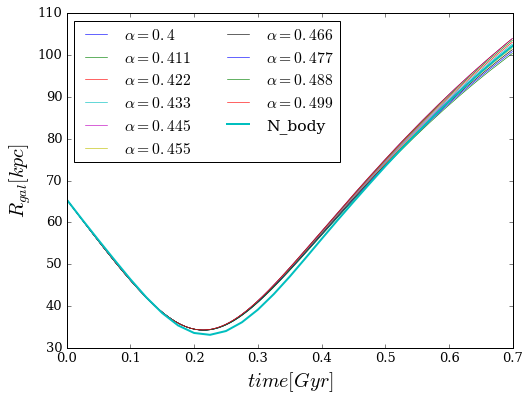
\includegraphics[scale=0.7]{../orbits_comparison_pos.png}
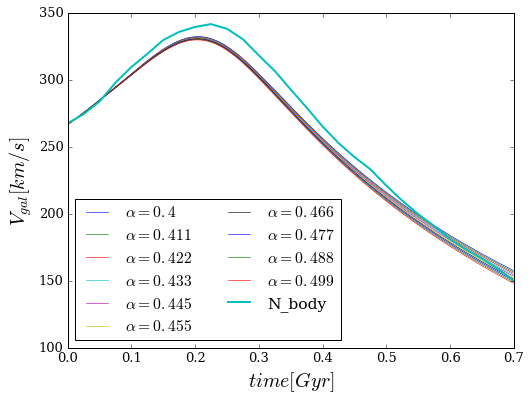
\includegraphics[scale=0.7]{../orbits_comparison_vel.png}
\caption{}
\end{figure}

The orbits for different $\alpha$ are shown in Fig.1, The best orbit is for $\alpha=0.44$
with this $\alpha$
the Sagittarius orbit was integrated backwards in time starting
from the initial conditions provided by Purcell \& Bullock and 
with the galaxy models provided in Gomez et al. Fig. 2 shows
the orbits of the sagittarius dwarf galaxy for $\alpha=1$
and $\alpha=0.44$. The initial conditions at $R_{vir}=261 kpc$
are summarized in table 2.

\begin{figure}
\centering
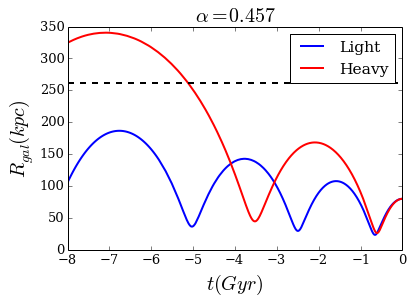
\includegraphics[scale=0.7]{sag_orbit_mdf.png}
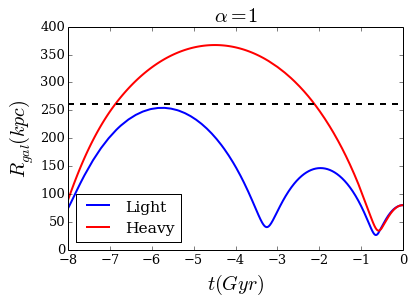
\includegraphics[scale=0.7]{sag_orbit.png}
\caption{}
\end{figure}

\begin{table}
\begin{tabular}{c c c c c c c}
\hline
Model & x(kpc) & y(kpc) & z(kpc) & vx(km/s) & vy(km/s) & vz(km/s) \\
\hline
${\alpha=1}$ & & & & & & \\
Light Sag &  -136.51 & 0 & 137.15 & 20.85 &  0 & -68.54  \\ 
MW & 7.03 & 0 & -80.19 & 15.5 & 0 & 39.85 \\
\hline
Heavy Sag & -146.13 & 0 & 145.19 & 25.02 & 0 & -78.74 \\
MW & 8.41 & 0 & -65.1& 12.42& 0 & 31.99\\
\hline
${\alpha=0.44}$ & & & & & & \\
Light Sag & -215.79  & 0 & -241.19 & 80.4 & 0 & 17.8 \\ 
MW & 9.93 & 0 & -110.18 & -10-03 & 0  & 33.68 \\
\hline
Heavy Sag & -209.06 & 0  & -225.62 & 88.17 & 0 & 17.44 \\
MW & 8.39 & 0 & -81.33 & -9.00 & 0 & 24.77\\
\hline
\end{tabular}
\caption{}
\end{table}
